\section{Stores Sesh (8 weeks to go!)}


\margininbox{Facebook Excuses}{
Given reasons for not coming on expo:
\begin{itemize}
    \item "If I skip this one, the next one will have less visa hassle" -- Thara Supasiti
    \item "riding the new bike after getting back from SA" -- Martin McGowan
    \item "going on a busking tour next month" and also "my bedroom ceiling just started leaking uncontrollably" therefore "my room has already turned into the bivvy" -- Rik Venn
    \item "Getting down \passage{avaline's} is about all I'm aspiring to this year!" -- Pete Jurd
\end{itemize}

Most honestly:

\begin{itemize}
    \item "Not attending due to poor life management skills." -- Andrew Mitchell
\end{itemize}}{\logbook}

I texted Jan just after midday, he was still in bed. Chastising him
gently \& signing off with a usual “to minus 1000” I get by way of
reply:

“I’m visualising -2000 – mental preparation is key”

With a typically ICCC alpine start, the day dragged on into festernoon and the workers assembled.

We checked out all the club tents — we have two A.OK Mk 4 F10s, for
that classic orange vibe, and the Equinox 450 (The Casino) actually
seems OK (no broken poles). Though all could do with a proof.

Three sets of (11,10,10mm Mammut) 200m rope were carefully chained in
the quad, and put in the soak.

Finally, Jan spent the afternoon assembling bits of our Raumer
Stick-Up into a working setup for bolt climbing. Our plan is to check
it and the drills out in Yorkshire in a couple of weekends time. For
now, however, we’ve had to make do with a hilarious ‘climbing the
north face of \passage{Beit Quad}’ with tent-pegs nicked from the tents as
pretend rawl bolts, checking that the lengths of the various etriers
agrees with what we can reach with the drill. 

\name{Jarvist Frost}


\subsection{Tent Proof, Approvedfood \& survey books}

\begin{marginfigure}
\checkoddpage \ifoddpage \forcerectofloat \else \forceversofloat \fi
\centering
 \frame{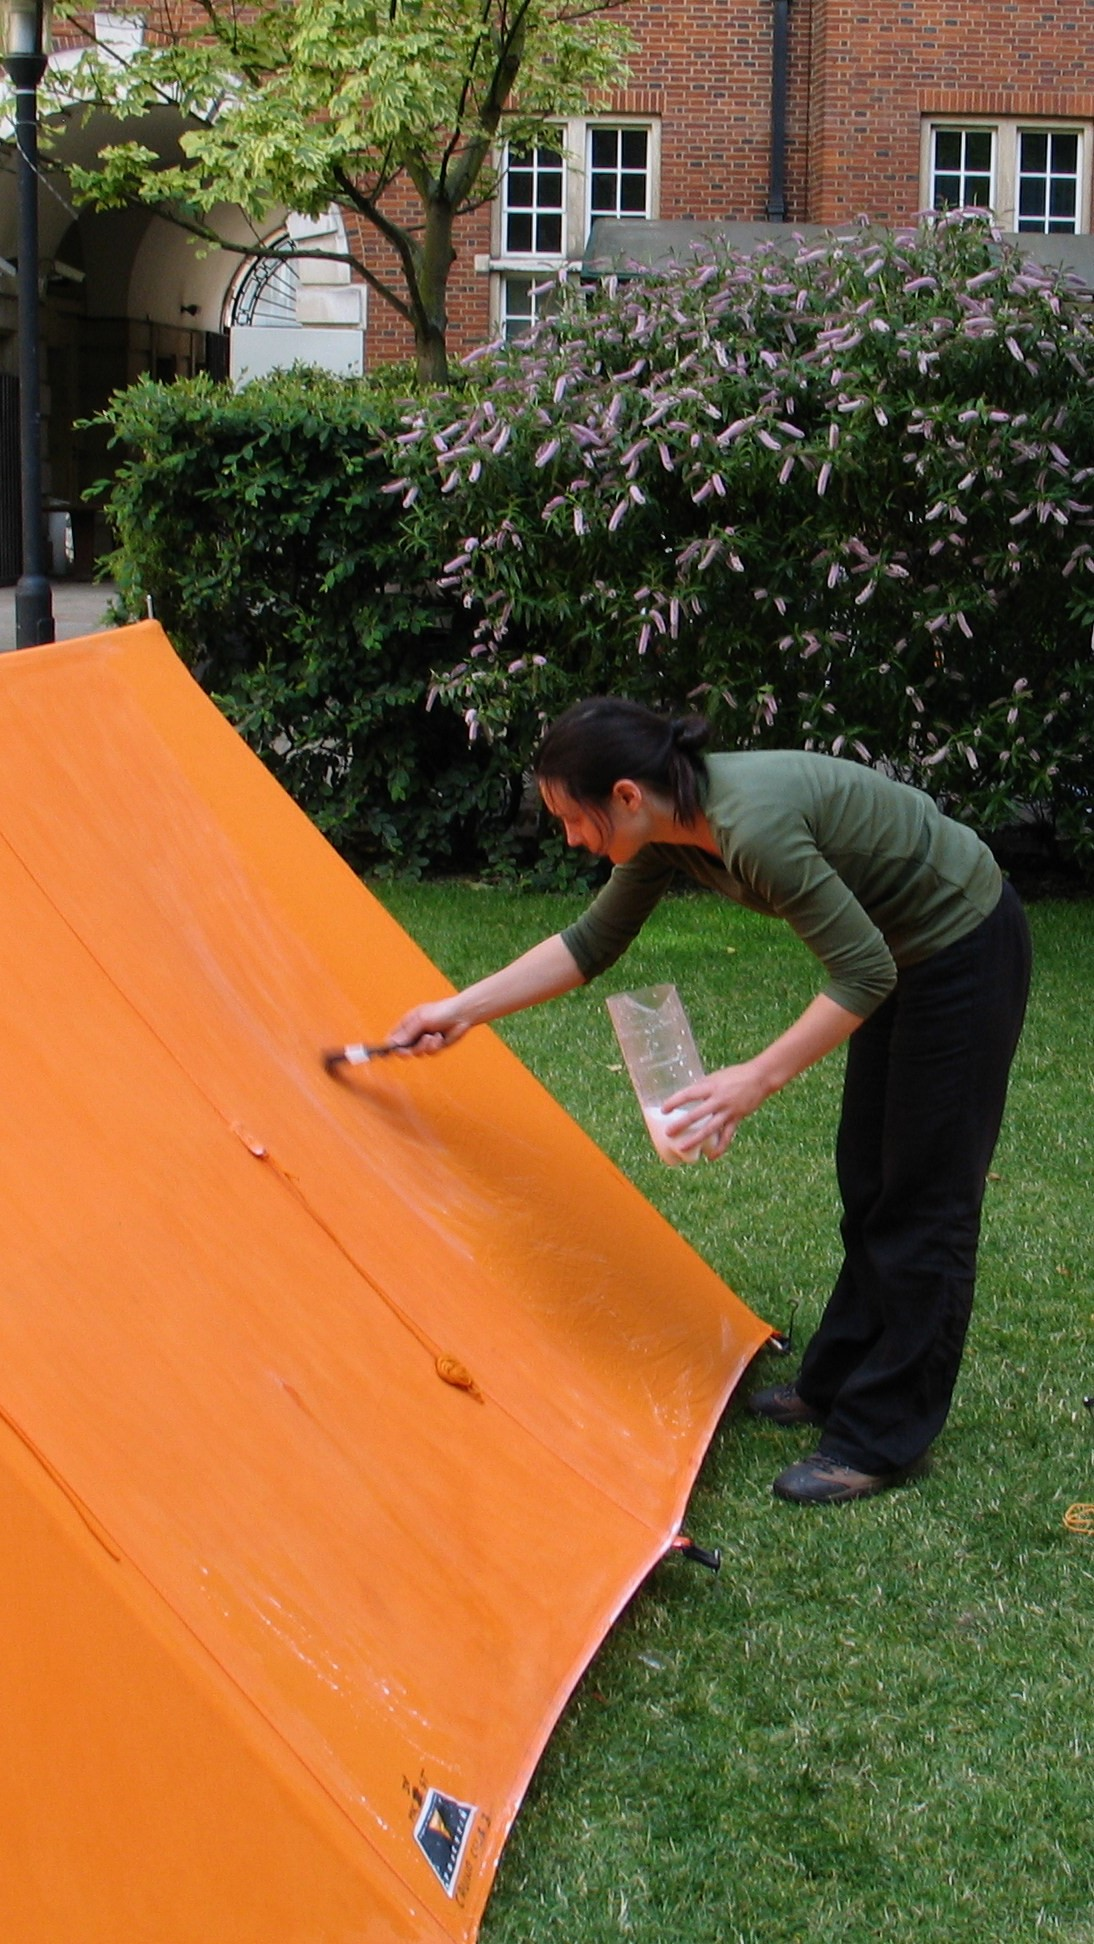
\includegraphics[width=\linewidth]{2011/stores/2011-06-19-15.57.05-Jarvist Frost-CanonG5-IMG_0014b - proofing tents--orig.jpg}} 
 \caption{Waterproofing the F10 tents in Beit Quad in June. \pic{Jarvist Frost}}
 \label{tentproofing}
\end{marginfigure}

Preparations grind slowly on; old F10s proofed with a paint brush
(Nikwax Cotton Proof), the Nylon tents spruced up with some Nikwax
Tent \& Gear proof.

We’ve bought quite a lot of food from http://approvedfood.co.uk, it’s
pretty cheap and the BB date is rather irrelevant when you food is
dried. Since we don’t have anyone with a personal car in London,
anything we can get the postie to bring is something we don’t have to
trawl around London \& acquire ourself! The usual fun of emptying multi
packs into green crates, splitting tins \& etc. was engaged on. It’s
amazing how dense you can pack when you really try, certainly the
Tetris practice comes in useful!

Finally, we got a load of new Gelert / BCB waterproof notebooks.
The paper’s really good for surveying, a properly waterproofed plastic
paper but with a surface rough enough to take a pencil mark easily.
Previously we’ve printed our own survey books with A4 Aquascribe
(a rag waterproof paper, so gets mud ingrained into it rather easily),
and old plotter paper (a bit too shiny, you really need a biro /
permanent marker, but then it's lovely), but now we’re having to stoop
to do it by hand. Pretty laborious! 
\name{Jarvist Frost}

\newpage

\subsection{T-7 days}


\begin{marginfigure}
\checkoddpage \ifoddpage \forcerectofloat \else \forceversofloat \fi
\centering
 \frame{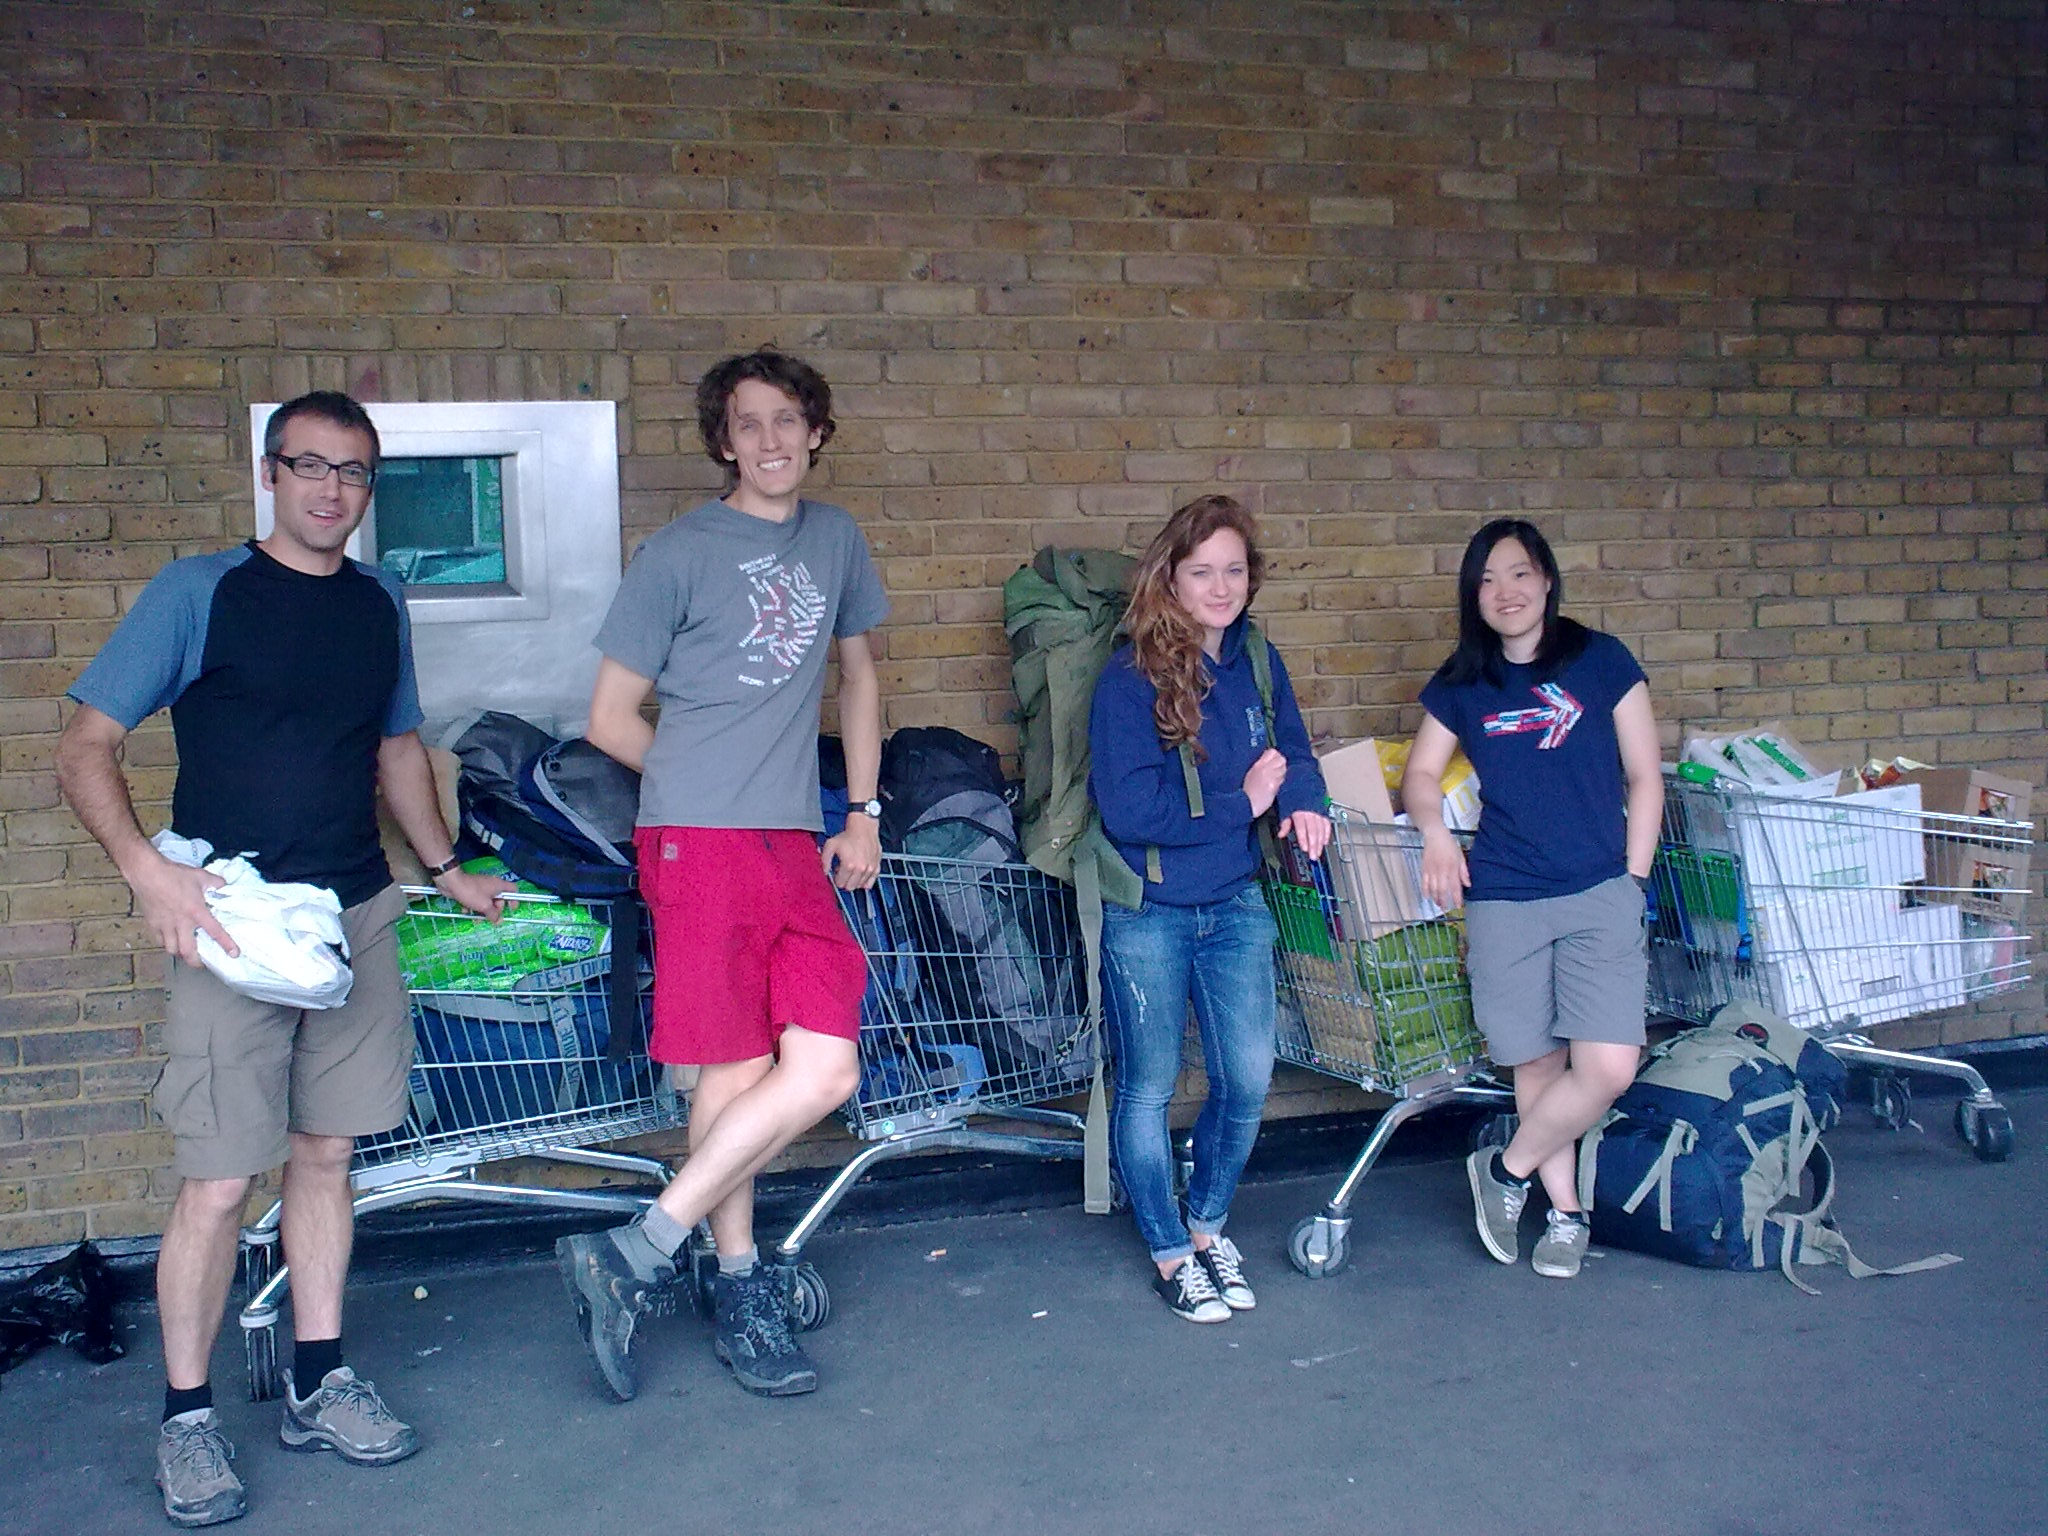
\includegraphics[width=\linewidth]{2011/stores/2011-07-02-12.40.03-Jana Carga-Camera Phone-Image0311--orig.jpg}} 
 \caption{Part of the shopping gang - Tetley, Jarv, Ari and Clare - after visiting ASDA and Lidl. \pic{Jana Čarga}}
 \label{food 2011}
\end{marginfigure}

On the day the last ever space shuttle blasts off, we’ve entered that
horrible time seven days or so before expedition when it’s suddenly
become too late to sort out anything major, yet there’s lots of
trivial jobs that need doing\ldots{} at some point. Just one last package
to arrive in the post, a new 80W solar panel to be used on the
mountain at the campsite, then transferred to the Slovenians for use
on the new mini mountain hut which is proposed to be flown up to Mig
this Autumn.

Still, last weekend we spent a full day around the ASDA and Lidl at
\passage[town]{Clapham Junction}, before abusing a taxi to transport our swag back to
\passage[town]{South Kensington}. After throwing away all the superfluous cardboard food
comes in, and packing it densely into green removals crates, we went
home exhausted. Returning on Sunday we cut rigging tape to length,
sorted all of our many (so many!) first aid kits and carefully doubled
bagged and densely stuffed underground camping gear into tackle sacks.
Our fairly sizeable stores are absolutely stuffed with crates, bags
and big blue barrels. How we fit it all in and on a 9-seater Transit I
will never truly understand.

Minor jobs proceeded during the week. This weekend we are finishing
off the shopping on Saturday (a hundred trivial things we can’t
survive without: peanut butter, soya mince, squeezy marmite etc.),
packing personal caving gear and sorting out all the rigging and
bolting equipment we need.

To this end my sitting room currently looks like some unholy cross
between caving stores and an electronics workshop. A smouldering
solder iron lurks in the corner, overseeing the contents of burst open
drills; the smell of rosin flux competing with the darker note of
Toluene rising off the patched oversuit on the floor. 


\begin{marginfigure}
\checkoddpage \ifoddpage \forcerectofloat \else \forceversofloat \fi
\centering
 \frame{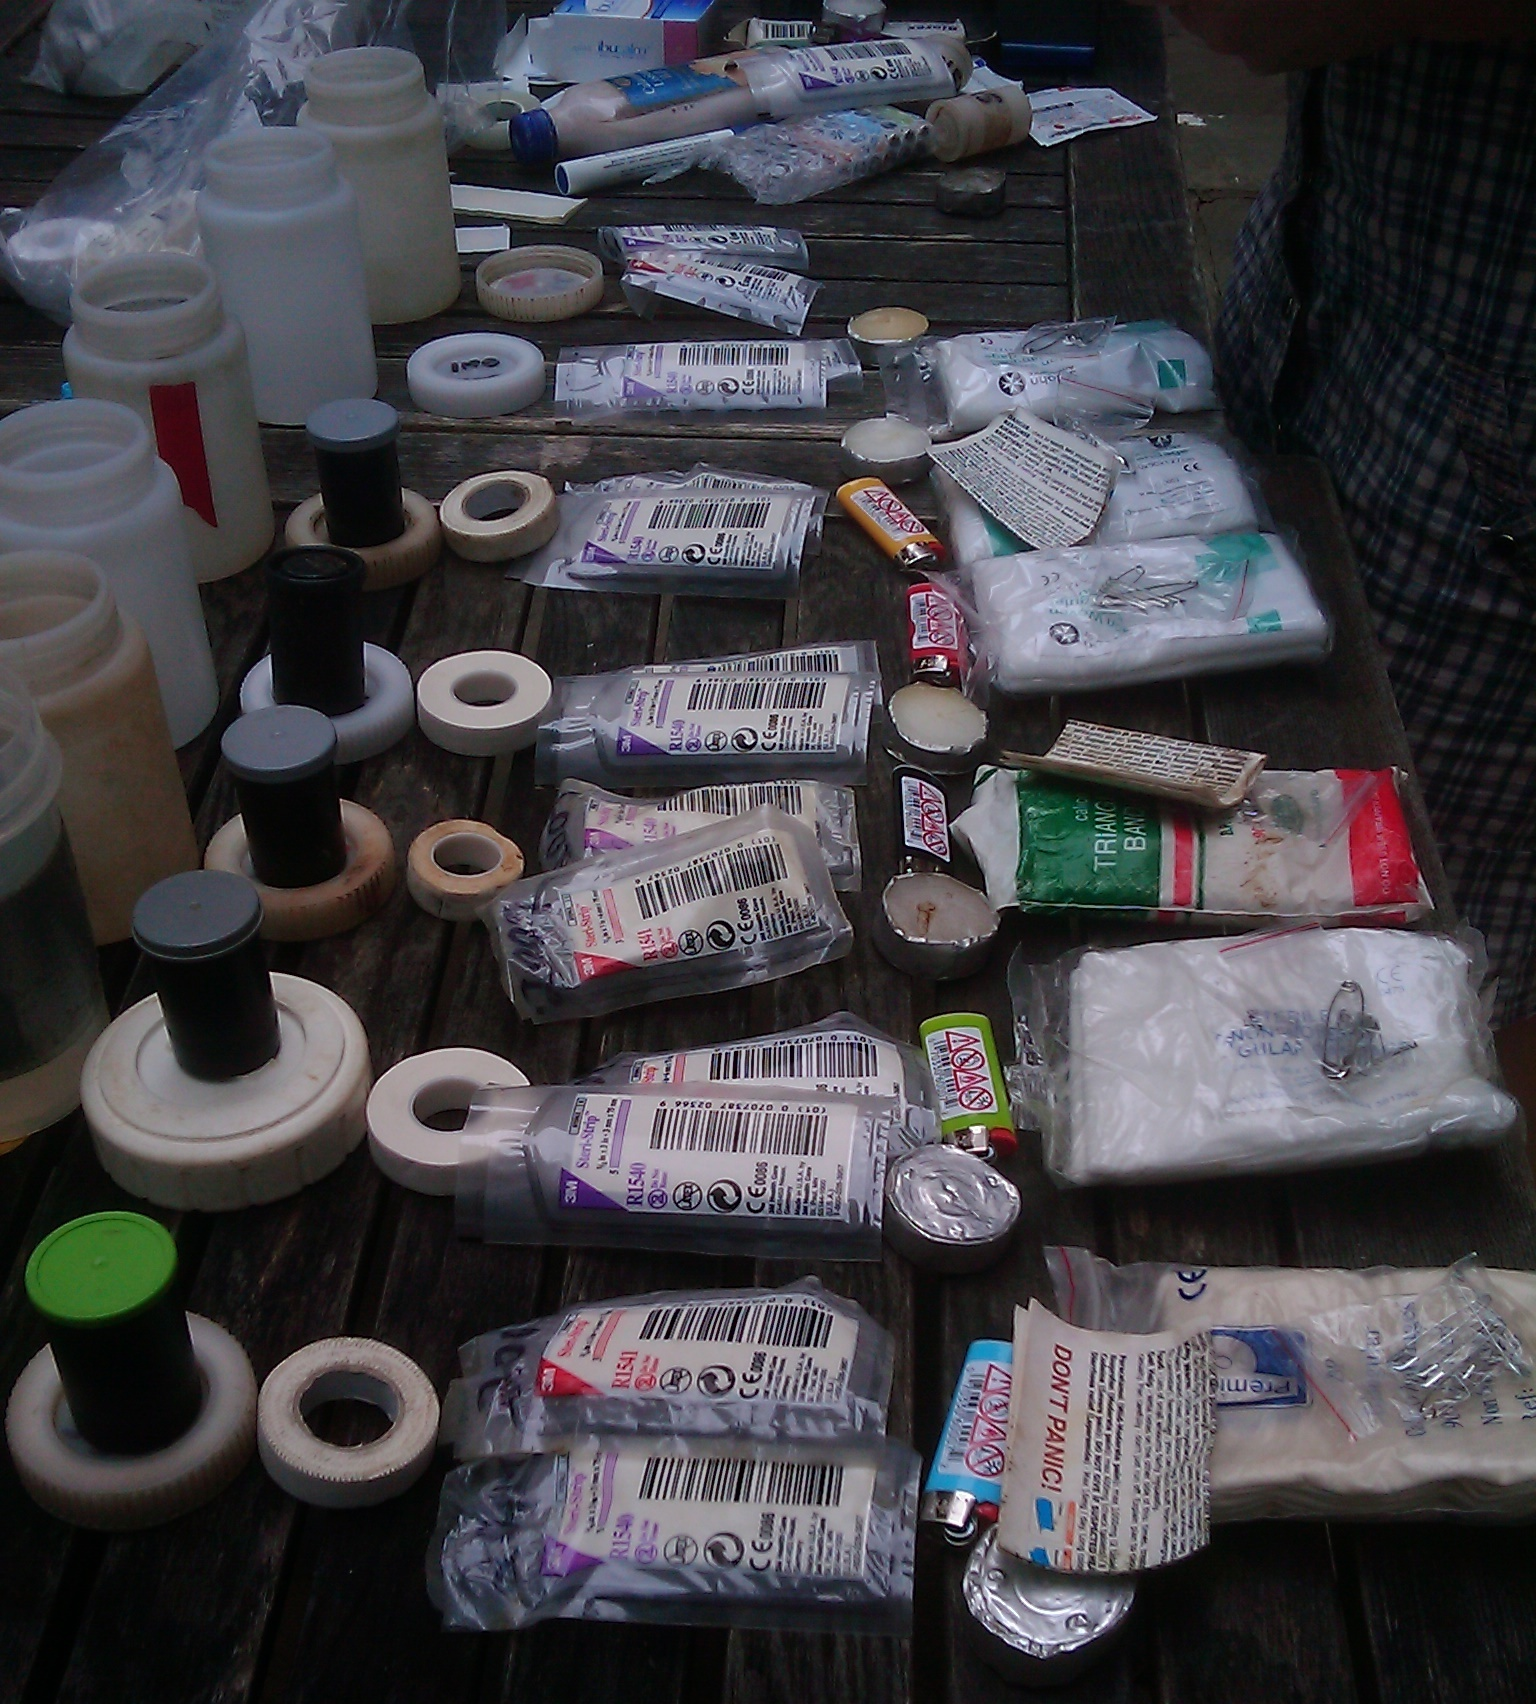
\includegraphics[width=\linewidth]{2011/stores/2011-07-03-16.08.00-Jan Evetts-Camera Phone-IMAG0327--orig.jpg}} 
 \caption{Preparing small first aid kits that can be carried on every caving trip. \pic{Jan Evetts}}
 \label{caving first aid}
\end{marginfigure}


From an organisational point of view I find these times very strange,
everything slowly going quiet as the ToDo list shrinks, itineraries
are filled, all bags are packed. Underground camp bags are ready to be
opened at -550 m, bolting kits are prepared, survey books are filled
with neat indelible guidelines, carefully washed and dried rope is
ready to spool out of bags while abseiling down hitherto undescended
shafts, shedding light on the walls for the first time in history.

Like some grotesque Hemulen in a Moomin novel just as the true raison d'etre of the expedition (the actual exploration of new cave) starts, the need for any further organisation disappears. Nothing left to do but lace up the walking boots, fill a bag and head up \passage[mountain]{Migovec} herself.

\name{Jarvist Frost}


\newpage
\begin{pagefigure}
\checkoddpage \ifoddpage \forcerectofloat \else \forceversofloat \fi
\frame{
\includegraphics[width=\linewidth]{2011/stores/migovec_cavers_expo.jpg}}
\caption{Expedition poster, using the famous "Lord Kitchener Wants You" World War I recruitment poster designed by Alfred Leete. Notably, Lord Kitchener is using an electric, not carbide, light. \pen{Jarvist Frost}} \label{kitchener wants you}
\end{pagefigure}